\documentclass[11pt,a4paper]{article}
\usepackage[utf8]{inputenc}
\usepackage[T1]{fontenc}
\usepackage[italian]{babel}
\usepackage{lmodern}
\usepackage[a4paper,margin=2.3cm]{geometry}
\usepackage{amsmath,amssymb}
\usepackage{graphicx}
\usepackage{booktabs}
\usepackage{tabularx}
\usepackage{multirow}
\usepackage{array}
\usepackage{float}
\usepackage{longtable}
\usepackage{caption}
\usepackage{enumitem}
\usepackage[hidelinks]{hyperref}
\usepackage{xcolor}

\graphicspath{{../figure/}}
\setlist{nosep,leftmargin=*}
\captionsetup{font=small,labelfont=bf}
\renewcommand{\arraystretch}{1.15}

% nuclide: \nuc{137}{Cs}
\newcommand{\nuc}[2]{\ensuremath{{}^{#1}\mathrm{#2}}}
\newcommand{\ee}[1]{\cdot 10^{#1}}
\newcommand{\pmm}{\,\pm\,}
\newcommand{\gam}{$\gamma$}
\newcommand{\keV}{\,keV}
\newcommand{\mcps}{\,mcps}

\title{Analisi di spettri \gam{} HPGe:\\ un campione di trinitite e un campione di lantanio metallico}
\author{}
\date{Novembre 2026}

\begin{document}
\maketitle

\begin{abstract}
\noindent
Sono stati analizzati due spettri \gam{} acquisiti con lo stesso spettrometro HPGe, uno di un frammento di trinitite e uno di un pezzo di lantanio metallico. I due campioni sono trattati in modo \emph{indipendente}: ogni spettro è valutato soltanto con informazioni interne a sé stesso.

Nella trinitite sono identificati \nuc{137}{Cs}, \nuc{241}{Am}, \nuc{152}{Eu}, \nuc{133}{Ba} e \nuc{239}{Pu}, mentre \nuc{60}{Co}, \nuc{154}{Eu} e \nuc{155}{Eu} non sono rivelabili, come atteso dopo 81~anni di decadimento. Con una calibrazione in efficienza relativa costruita sul \nuc{152}{Eu} del campione, il rapporto di attività \nuc{137}{Cs}/\nuc{152}{Eu}, riportato alla data della detonazione, vale $5{,}7\pm0{,}3$.

Il lantanio metallico, di composizione isotopica naturale, mostra le due linee del \nuc{138}{La} e la catena completa dell'\nuc{227}{Ac} in equilibrio secolare. Usando il \nuc{138}{La} come riferimento interno si ottengono $A(\nuc{227}{Ac})/A(\nuc{138}{La})\approx1{,}4$--$1{,}7$, cioè circa $1{,}1$--$1{,}4$\,Bq di \nuc{227}{Ac} per grammo di La.
\end{abstract}

\section{Dati sperimentali e limiti dell'analisi}

Gli spettri sono stati acquisiti con GammaVision~6.08 e un MCA Easy-MCA-2k (SN~15043603), su 2048 canali da circa $1{,}385$\,keV/canale, coprendo l'intervallo 0--2840\,keV.

\begin{table}[H]
\centering\small
\resizebox{\textwidth}{!}{%
\begin{tabular}{llllll}
\toprule
File & Campione & Inizio misura & Live time & Real time & Tempo morto\\
\midrule
\texttt{Sabbia\_vetrificata\ldots.Spe} & trinitite & 21/10/2026 16:47:45 & 91\,070\,s (25,3\,h) & 91\,083\,s & $\approx0{,}01\%$\\
\texttt{Lantan\ldots.Spe} & La metallico & 28/10/2026 11:04:28 & 113\,768\,s (31,6\,h) & 113\,777\,s & $\approx0{,}01\%$\\
\bottomrule
\end{tabular}}
\end{table}

Per nessuna delle due misure sono disponibili una calibrazione in efficienza, uno spettro di fondo, la massa del campione o la geometria di misura. Di conseguenza non si riportano attività assolute. Si riportano invece:
\begin{enumerate}[label=(\roman*)]
\item i nuclidi identificati, con i tassi netti di conteggio;
\item i rapporti di attività ottenuti con una calibrazione in efficienza relativa \emph{interna} al campione;
\item i limiti di rivelabilità per i nuclidi attesi ma non osservati.
\end{enumerate}

\section{Metodo}

\paragraph{Calibrazione in energia.}
I file contengono la calibrazione di GammaVision, $E=-0{,}050+1{,}38516\,c+7{,}3\ee{-7}c^2$, con $c$ il numero di canale. L'ho verificata e rifittata con picchi di riferimento noti, ottenendo
\[
E\,[\mathrm{keV}] = 0{,}193 + 1{,}38546\,c + 5{,}34\ee{-7}\,c^2,
\]
con residui $\le0{,}3$\,keV ($\le0{,}2$ canali).

\paragraph{Risoluzione.}
La larghezza dei picchi segue
\[
\mathrm{FWHM}^2 = 0{,}925 + 2{,}14\ee{-3}\,E \quad [\mathrm{keV}^2],
\]
cioè circa $1{,}5$\,keV a 662\,keV e circa $2{,}0$\,keV a 1332\,keV. Con $1{,}385$\,keV/canale ogni picco occupa solo 1--2 canali (forte sotto-campionamento), e i doppietti più vicini di circa $1{,}5$\,keV non si separano.

\paragraph{Fit dei picchi.}
Ogni picco è descritto da una gaussiana integrata sul canale, più un fondo lineare locale. Il fit usa minimi quadrati pesati iterati, che approssimano la verosimiglianza di Poisson, e i multipletti sono fittati simultaneamente. Le energie sono fissate ai valori di libreria, con uno spostamento comune ammesso di $\pm0{,}8$\,keV e un fattore di scala della larghezza tra $0{,}8$ e $1{,}4$. Per ciascun campione si usa una libreria dedicata, completata dalle linee del fondo naturale (serie di U e Th, \nuc{40}{K}) e dai raggi~X del Pb.

\paragraph{Criteri di decisione.}
Si adottano i criteri di Currie, $L_C=2{,}33\sqrt{B}$ e $L_D=2{,}71+4{,}65\sqrt{B}$, dove $B$ è il fondo sotto $\pm3\sigma$ del picco. Un picco è considerato rivelato se la sua area netta supera sia $L_C$ sia $3\sigma$. Una scansione canale per canale cerca inoltre eccessi $>4\sigma$ non assegnati.

\paragraph{Dati nucleari e codice.}
Energie e intensità \gam{} sono tratte da ENSDF/NNDC e DDEP/LNHB. Codice, tabelle complete (\texttt{picchi\_*.csv}) e log sono nella cartella \texttt{analisi\_HPGe/}.

%=====================================================================
\section{Parte A --- Trinitite}

\begin{figure}[H]
\centering
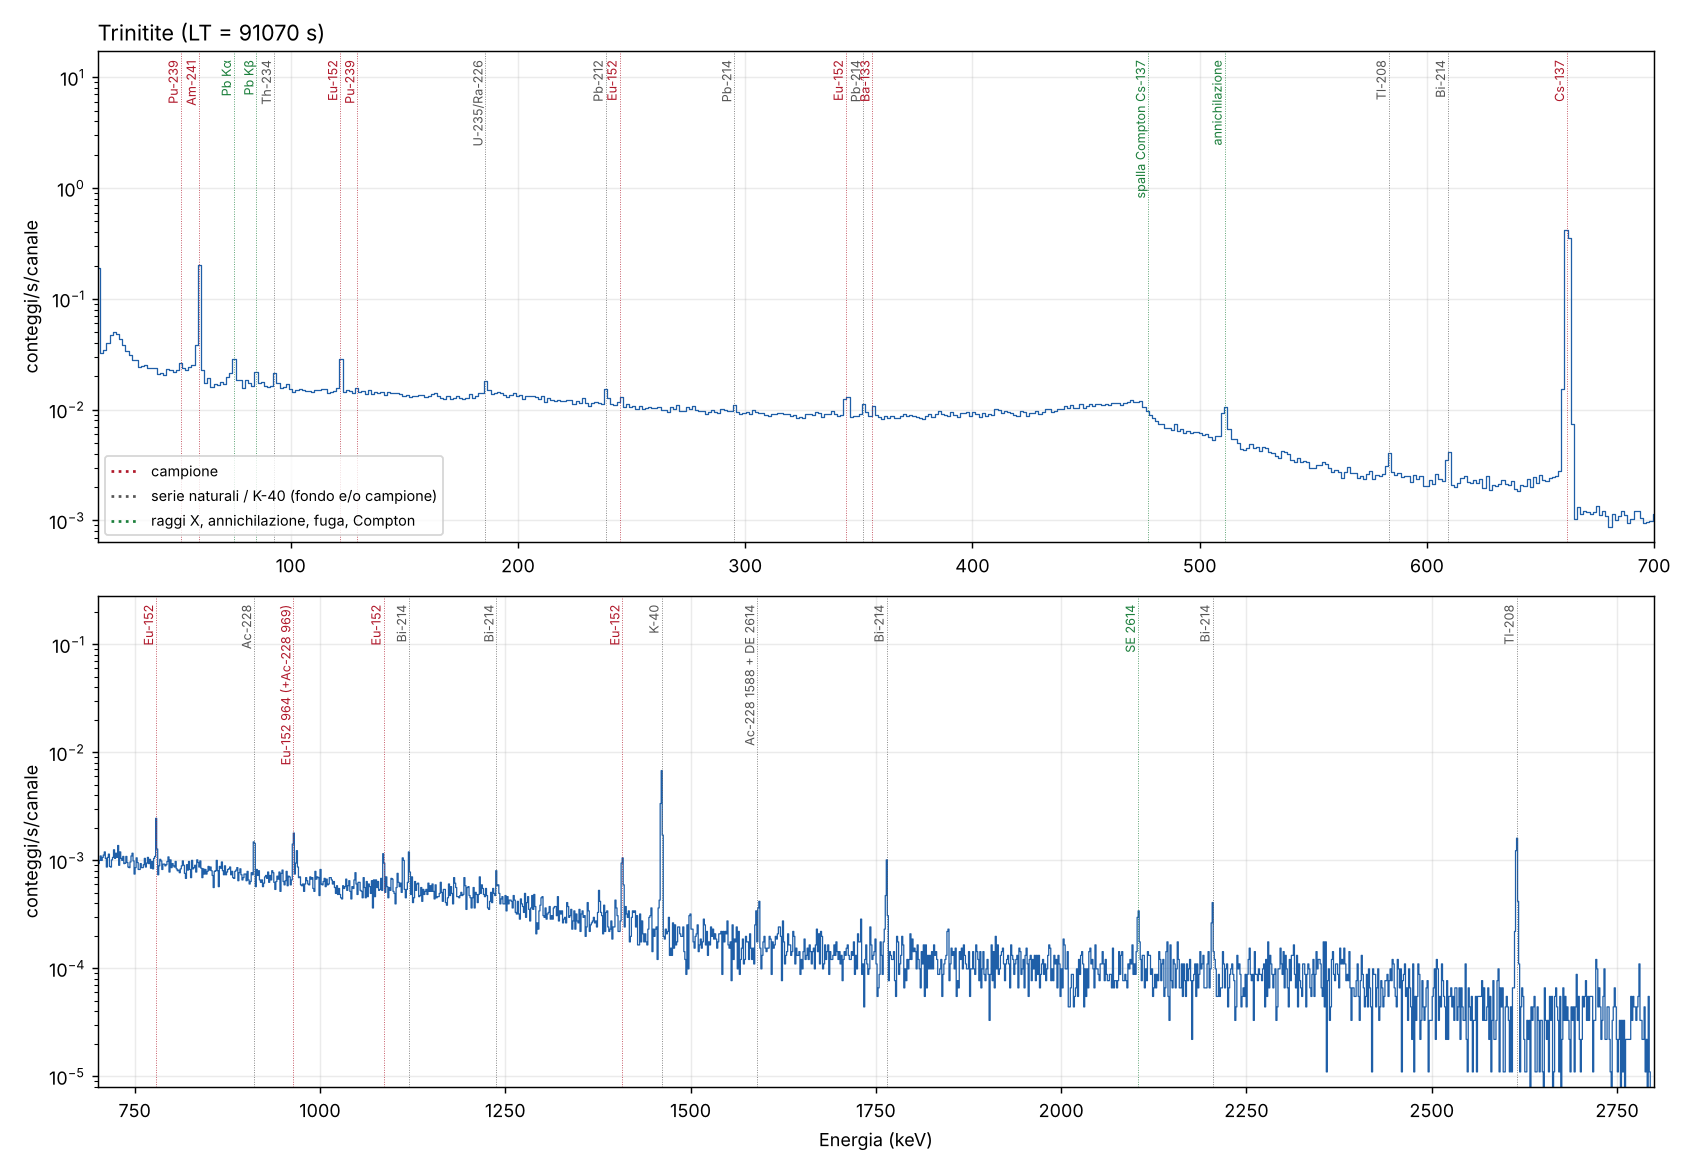
\includegraphics[width=\textwidth]{fig1_spettro_trinitite.png}
\caption{Spettro della trinitite, normalizzato al live time.}
\end{figure}

\subsection{Nuclidi identificati}

\begin{table}[H]
\centering\small
\resizebox{\textwidth}{!}{%
\begin{tabular}{lllrrl}
\toprule
Nuclide & $T_{1/2}$ & Linea [keV] ($I_\gamma$\,\%) & Tasso netto [mcps] & Sign. & Origine\\
\midrule
\nuc{137}{Cs} & 30,08\,a & 661,66 (85,1) & $789{,}1\pm3{,}0$ & $>250\sigma$ & prodotto di fissione\\
\nuc{241}{Am} & 432,6\,a & 59,54 (35,9) & $197{,}9\pm1{,}6$ & $>100\sigma$ & da \nuc{241}{Pu} del combustibile\\
\multirow{7}{*}{\nuc{152}{Eu}} & \multirow{7}{*}{13,52\,a} & 121,78 (28,5) & $15{,}5\pm0{,}6$ & $25\sigma$ & \multirow{7}{*}{\nuc{151}{Eu}(n,$\gamma$) nel suolo}\\
 & & 244,70 (7,6) & $3{,}0\pm0{,}5$ & $6\sigma$ & \\
 & & 344,28 (26,6) & $6{,}9\pm0{,}6$ & $12\sigma$ & \\
 & & 778,90 (12,9) & $2{,}05\pm0{,}21$ & $10\sigma$ & \\
 & & 964,08 (14,5) & $1{,}74\pm0{,}22^{*}$ & $8\sigma$ & \\
 & & 1085,84 (10,1) & $0{,}99\pm0{,}16$ & $6\sigma$ & \\
 & & 1408,01 (20,9) & $1{,}68\pm0{,}18$ & $9\sigma$ & \\
\multirow{2}{*}{\nuc{133}{Ba}} & \multirow{2}{*}{10,55\,a} & 356,01 (62,1) & $2{,}08\pm0{,}42$ & $5\sigma$ & \multirow{2}{*}{\nuc{132}{Ba}(n,$\gamma$)}\\
 & & 302,85 (18,3) & $0{,}82\pm0{,}45$ & $<2\sigma$ & \\
\multirow{2}{*}{\nuc{239}{Pu}} & \multirow{2}{*}{24\,110\,a} & 51,62 (0,0272) & $3{,}6\pm0{,}7$ & $5{,}4\sigma$ & \multirow{2}{*}{combustibile non fissionato}\\
 & & 129,30 (0,0063) & $1{,}7\pm0{,}5$ & $3{,}1\sigma$ & \\
\bottomrule
\end{tabular}}
\caption{Nuclidi identificati nella trinitite. ${}^{*}$La linea a 964,08\,keV non è risolta dal \nuc{228}{Ac} a 964,77\,keV. Il contributo del \nuc{228}{Ac} è stimato dalla sua linea a 968,97\,keV nello stesso spettro, con il rapporto di intensità 4,99/15,8, e poi sottratto.}
\end{table}

\paragraph{Note sull'identificazione.}
\begin{itemize}
\item Le linee del \nuc{152}{Eu} a 411,1\,keV (interferenza non risolta) e a 1112,1\,keV (doppietto con \nuc{214}{Bi} a 1120,3\,keV) sono escluse dalla quantificazione.
\item \textbf{\nuc{239}{Pu}.}
\begin{itemize}
\item A 51,6\,keV non cade nessun'altra linea attesa tra i nuclidi presenti. I picchi di fuga del Ge dell'\nuc{241}{Am} si trovano a 49,7 e 48,6\,keV e sono distinti.
\item Il rapporto fra le due linee è coerente: dato il 51,6\,keV osservato, il 129,3\,keV atteso è 0,8--1,7\,mcps, e quello misurato è $1{,}7\pm0{,}5$\,mcps.
\item Le linee a 375,0 e 413,7\,keV ($I_\gamma\approx0{,}0015\%$) sono sotto il limite di rivelabilità, come atteso.
\item In letteratura il \nuc{239}{Pu} nella trinitite risulta osservabile in \gam{} ma difficile da quantificare~\cite{nist2021}.
\end{itemize}
In conclusione l'identificazione è solida, mentre la quantificazione resta indicativa.
\item \textbf{\nuc{133}{Ba}.} Il picco a 356\,keV è fittato insieme al \nuc{214}{Pb} a 351,9\,keV. Le linee secondarie (81, 303, 384\,keV) sono compatibili ma non significative. L'identificazione è quindi probabile, con significatività moderata.
\item Tutti i picchi dello spettro, compresi quelli non dovuti al campione, sono elencati e assegnati nella Tabella~\ref{tab:tuttiTR} (\S\ref{sec:tuttiTR}).
\end{itemize}

\begin{figure}[H]
\centering
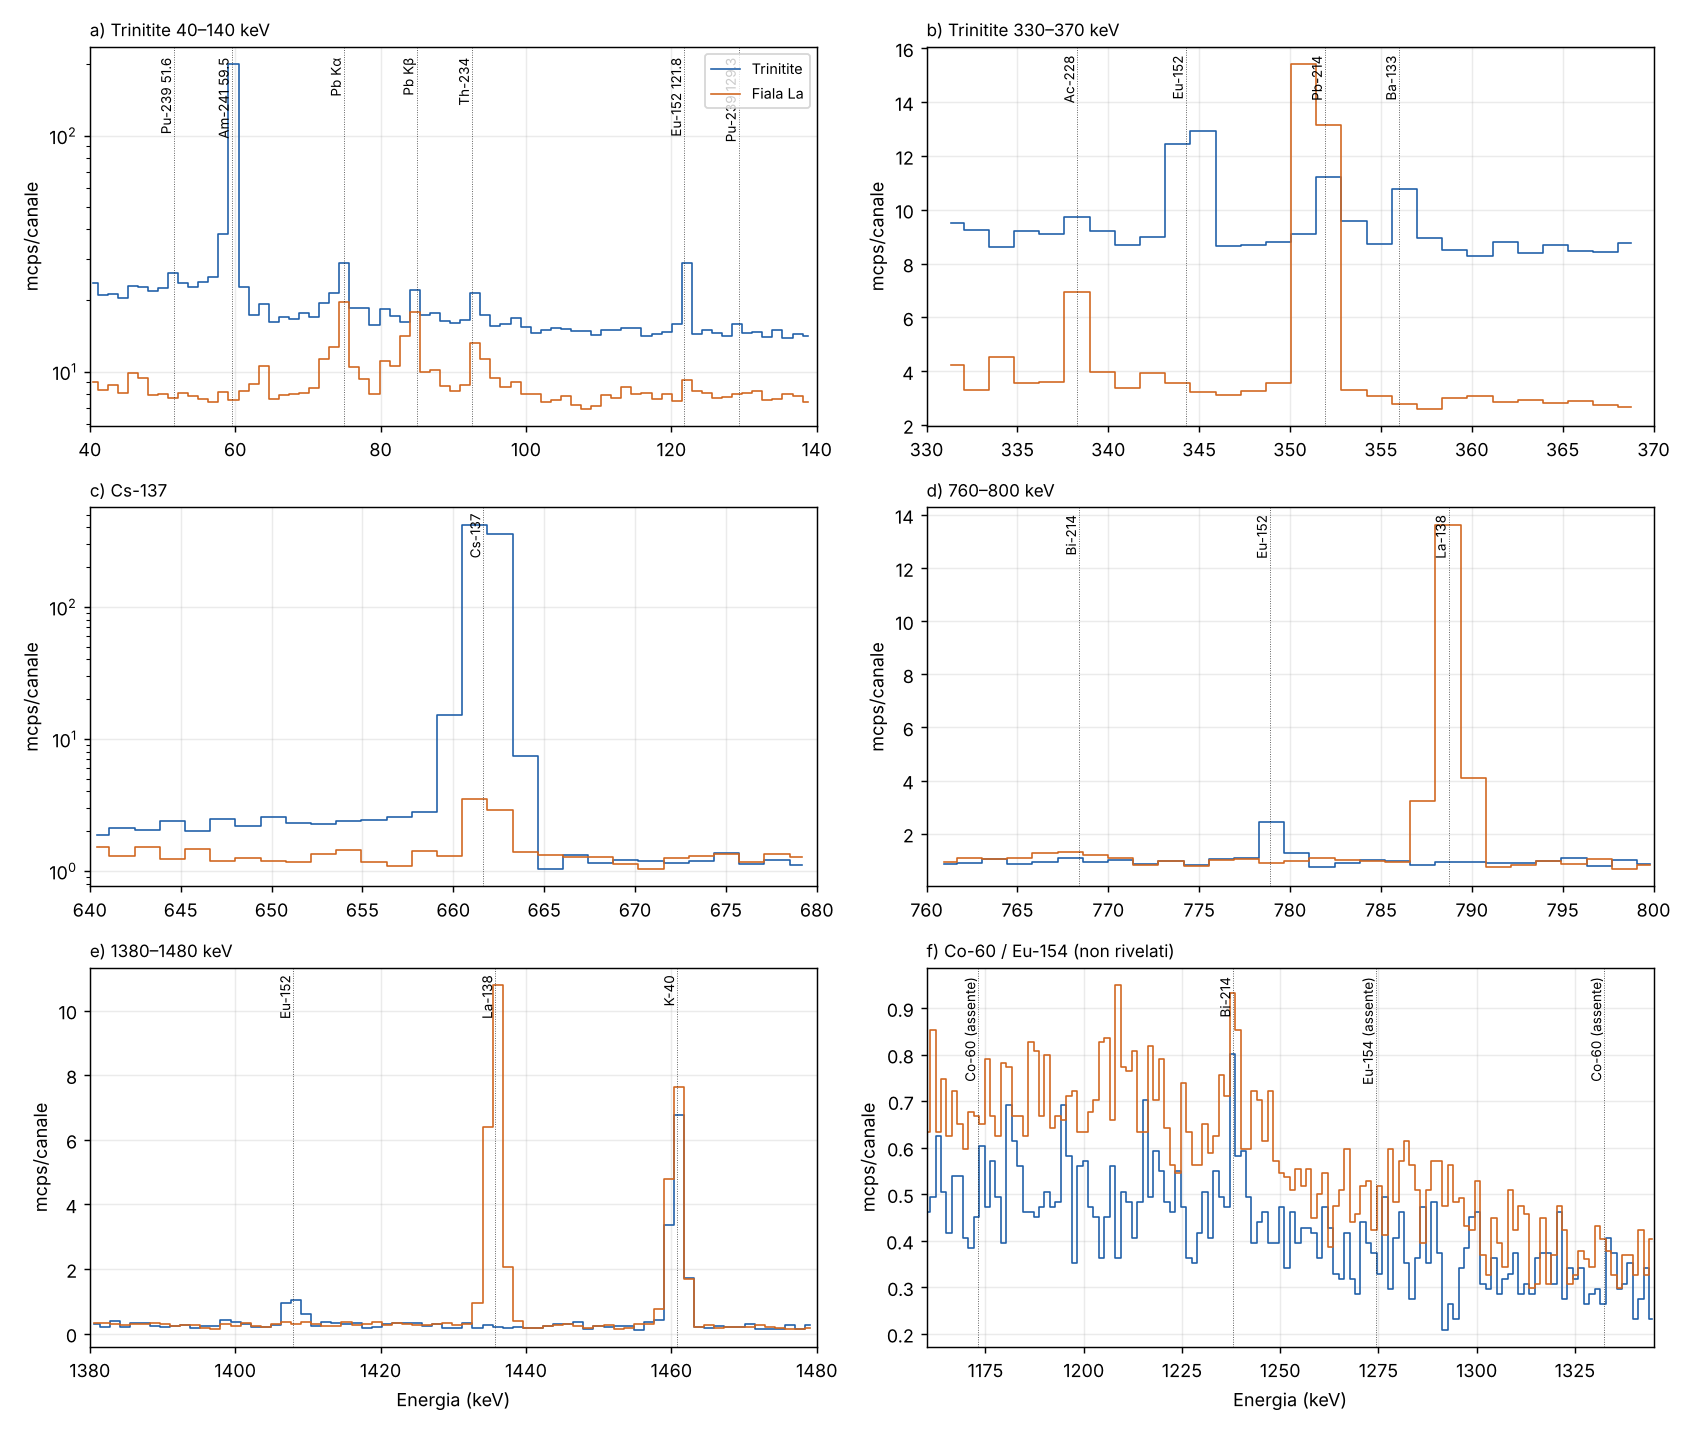
\includegraphics[width=\textwidth]{fig2_zoom_trinitite.png}
\caption{Trinitite, dettagli dello spettro: (a)~\nuc{239}{Pu} 51,6\,keV, \nuc{241}{Am}, \nuc{152}{Eu} 121,8\,keV, \nuc{239}{Pu} 129,3\,keV; (b)~\nuc{152}{Eu} 344\,keV e \nuc{133}{Ba} 356\,keV; (c)~\nuc{137}{Cs}; (d)~\nuc{152}{Eu} 778,9\,keV; (e)~\nuc{152}{Eu} 1408\,keV; (f)~regione di \nuc{60}{Co} e \nuc{154}{Eu}, dove non si osservano picchi.}
\end{figure}

\subsection{Nuclidi attesi ma non rivelati}

\begin{table}[H]
\centering\small
\resizebox{\textwidth}{!}{%
\begin{tabular}{llll}
\toprule
Nuclide & $T_{1/2}$ & Decadimento dal 16/07/1945 & Esito\\
\midrule
\nuc{60}{Co} & 5,27\,a & $2{,}3\ee{-5}$ & 1332,5\,keV $<0{,}49$\,mcps ($L_D$); $A/A(\nuc{152}{Eu})<0{,}06$\\
\nuc{154}{Eu} & 8,60\,a & $1{,}4\ee{-3}$ & 1274,4\,keV $<0{,}55$\,mcps; $A/A(\nuc{152}{Eu})<0{,}17$\\
\nuc{155}{Eu} & 4,75\,a & $7\ee{-6}$ & 86,5 e 105,3\,keV non rivelati\\
\bottomrule
\end{tabular}}
\end{table}

Il \nuc{152}{Eu} ha decaduto di un fattore $0{,}0155$ dal 1945. Rispetto ad esso, il \nuc{154}{Eu} ha perso un ulteriore fattore $0{,}09$ e il \nuc{60}{Co} un fattore $1{,}5\ee{-3}$. L'assenza di questi nuclidi dopo 81~anni è quindi attesa. Nei lavori di 20 o più anni fa erano invece riportati come presenti~\cite{parekh2006,belloni2011,core}.

\subsection{Rapporti di attività}

La curva di efficienza relativa è costruita sulle 7 linee pulite del \nuc{152}{Eu} del campione. Il modello è $\ln\varepsilon$ come polinomio di secondo grado in $\ln E$, con $\chi^2_\mathrm{rid}=0{,}6$. Geometria e autoassorbimento del frammento sono così inclusi nella curva.

Il rapporto di attività tra un nuclide $x$ e il \nuc{152}{Eu} si ottiene come
\[
\frac{A_x}{A_\mathrm{Eu}}=\frac{R_x}{I_{\gamma,x}\,\varepsilon_\mathrm{rel}(E_x)},
\]
dove $R_x$ è il tasso netto e $I_{\gamma,x}$ l'intensità della linea.

\begin{table}[H]
\centering\small
\begin{tabular}{lcc}
\toprule
Rapporto & al 21/10/2026 & al 16/07/1945 ($\Delta t=81{,}27$\,a)\\
\midrule
$A(\nuc{137}{Cs})/A(\nuc{152}{Eu})$ & $56\pm3$ & $\mathbf{5{,}7\pm0{,}3}$\\
$A(\nuc{133}{Ba})/A(\nuc{152}{Eu})$ & $0{,}12\pm0{,}03$ & $0{,}40\pm0{,}08$\\
$A(\nuc{239}{Pu})/A(\nuc{241}{Am})$ & $\approx24$--$34$ (indicativo) & ---\\
\bottomrule
\end{tabular}
\end{table}

Le incertezze riportate sono solo statistiche e di fit. Restano fuori tre effetti sistematici:
\begin{itemize}
\item la somma per coincidenza delle linee in cascata del \nuc{152}{Eu}. Senza conoscere la geometria non è quantificabile; in geometria ravvicinata va da qualche percento al 10--20\%. Il \nuc{137}{Cs} non ne è affetto;
\item per il rapporto Pu/Am, il rapporto di efficienza $\varepsilon(51{,}6)/\varepsilon(59{,}5)$, assunto tra 0,7 e 1,0;
\item un eventuale contributo di \nuc{137}{Cs} dal fondo ambientale, che senza uno spettro di fondo non è stato sottratto.
\end{itemize}

\subsection{Interpretazione}

\begin{itemize}
\item La combinazione osservata (\nuc{137}{Cs}, \nuc{152}{Eu}, \nuc{133}{Ba}, \nuc{241}{Am}, \nuc{239}{Pu}) è quella della trinitite del test Trinity descritta in letteratura~\cite{parekh2006,belloni2011,nist2021,core,jrnc2013}. Contiene un prodotto di fissione, prodotti di attivazione neutronica del suolo e del dispositivo, e il combustibile Pu con il suo discendente \nuc{241}{Am}.
\item L'\nuc{241}{Am} deriva in gran parte dal decadimento del \nuc{241}{Pu}, presente nel combustibile o prodotto per cattura neutronica durante la detonazione~\cite{nist2021}. Su 49~campioni, l'\nuc{241}{Am} riportato alla data della detonazione varia fra 1 e 42\,Bq/g~\cite{jrnc2013}.
\item Il \nuc{133}{Ba} è attribuito soprattutto all'attivazione del Ba contenuto nel Baratol, l'esplosivo convenzionale del dispositivo~\cite{nist2021}, con un possibile contributo del Ba delle sabbie arcosiche~\cite{jrnc2013}.
\item Il rapporto \nuc{137}{Cs}/\nuc{152}{Eu} varia molto da campione a campione. Tra prodotti di attivazione del suolo e radionuclidi del dispositivo non si osservano correlazioni~\cite{jrnc2013}, e il valore dipende tra l'altro dalla posizione rispetto al ground zero~\cite{belloni2011}. Il valore trovato caratterizza questo frammento e non va usato come prova di autenticità.
\end{itemize}

\subsection{Elenco completo dei picchi}\label{sec:tuttiTR}

La Tabella~\ref{tab:tuttiTR} riporta \emph{tutti} i picchi dello spettro della trinitite. Comprende i picchi trovati dalla scansione automatica con significatività $>4\sigma$ e le linee più deboli che risultano significative nel fit multiplo. Ogni picco è assegnato a una di quattro categorie:
\begin{itemize}
\item \textbf{C}: campione (radionuclidi del test Trinity);
\item \textbf{N}: radionuclidi naturali (serie di U e Th, \nuc{40}{K}). Senza uno spettro di fondo non si può distinguere quanto provenga dal frammento e quanto dall'ambiente;
\item \textbf{X}: raggi~X di fluorescenza dello schermo e picco di annichilazione;
\item \textbf{S}: strutture strumentali (picchi di fuga singola e doppia, spalla Compton).
\end{itemize}
Non restano picchi senza assegnazione. La Figura~1 riporta le stesse etichette.

{\small
\begin{longtable}{>{\raggedleft\arraybackslash}p{1.7cm}p{4.3cm}p{4.6cm}>{\raggedleft\arraybackslash}p{2.9cm}c}
\caption{Trinitite: elenco completo dei picchi e loro assegnazione. Tassi netti dal fit multiplo.}\label{tab:tuttiTR}\\
\toprule
$E$ [keV] & Assegnazione & Note & Tasso [mcps] & Cat.\\
\midrule\endfirsthead
\toprule
$E$ [keV] & Assegnazione & Note & Tasso [mcps] & Cat.\\
\midrule\endhead
\bottomrule\endfoot
$<30$ & soglia del discriminatore & 15,4\,keV: picco sul primo canale utile; nessun picco risolvibile & --- & S\\
51,6 & \nuc{239}{Pu} & & $3{,}6\pm0{,}7$ & C\\
59,5 & \nuc{241}{Am} & & $197{,}9\pm1{,}6$ & C\\
72,8 / 75,0 & Pb K$\alpha_2$ / K$\alpha_1$ & fluorescenza dello schermo & $6{,}6\pm0{,}7$ / $12{,}9\pm0{,}6$ & X\\
84,9 / 87,3 & Pb K$\beta_1$ / K$\beta_2$ & fluorescenza dello schermo & $6{,}8\pm0{,}7$ / $2{,}3\pm0{,}7$ & X\\
92,6 & \nuc{234}{Th} (92,4 + 92,8) & serie \nuc{238}{U} & $\approx5{,}5$ & N\\
121,8 & \nuc{152}{Eu} & & $15{,}5\pm0{,}6$ & C\\
129,3 & \nuc{239}{Pu} & & $1{,}7\pm0{,}5$ & C\\
185,7 & \nuc{235}{U} + \nuc{226}{Ra} (186,2) & & $6{,}3\pm0{,}6$ & N\\
238,6 & \nuc{212}{Pb} & serie \nuc{232}{Th} & $6{,}1\pm0{,}6$ & N\\
244,7 & \nuc{152}{Eu} & & $3{,}0\pm0{,}5$ & C\\
295,2 & \nuc{214}{Pb} & serie \nuc{238}{U} & $1{,}9\pm0{,}4$ & N\\
344,3 & \nuc{152}{Eu} & & $6{,}9\pm0{,}6$ & C\\
351,9 & \nuc{214}{Pb} & serie \nuc{238}{U} & $2{,}2\pm0{,}4$ & N\\
356,0 & \nuc{133}{Ba} & & $2{,}1\pm0{,}4$ & C\\
411,1 & \nuc{152}{Eu} & interferenza non risolta & $1{,}9\pm0{,}5$ & C\\
$\sim$477 & spalla Compton del \nuc{137}{Cs} & $E_C=477{,}3$\,keV; non è un picco & --- & S\\
511,0 & annichilazione + \nuc{208}{Tl} 510,8 & & $10{,}5\pm0{,}6$ & X/N\\
583,2 & \nuc{208}{Tl} & serie \nuc{232}{Th} & $2{,}2\pm0{,}3$ & N\\
609,3 & \nuc{214}{Bi} & serie \nuc{238}{U} & $3{,}1\pm0{,}3$ & N\\
661,7 & \nuc{137}{Cs} & & $789{,}1\pm3{,}0$ & C\\
778,9 & \nuc{152}{Eu} & & $2{,}05\pm0{,}21$ & C\\
911,2 & \nuc{228}{Ac} & serie \nuc{232}{Th} & $1{,}55\pm0{,}19$ & N\\
964,1 & \nuc{152}{Eu} (+ \nuc{228}{Ac} 964,8) & & $1{,}74\pm0{,}22$ & C\\
969,0 & \nuc{228}{Ac} & & $1{,}06\pm0{,}18$ & N\\
1085,8 & \nuc{152}{Eu} & & $0{,}99\pm0{,}16$ & C\\
1112,1 & \nuc{152}{Eu} & doppietto con 1120,3 & $0{,}77\pm0{,}16$ & C\\
1120,3 & \nuc{214}{Bi} & & $0{,}79\pm0{,}16$ & N\\
1238,1 & \nuc{214}{Bi} & & $0{,}49\pm0{,}13$ & N\\
1377,7 & \nuc{214}{Bi} & & $0{,}45\pm0{,}12$ & N\\
1408,0 & \nuc{152}{Eu} & & $1{,}68\pm0{,}18$ & C\\
1460,8 & \nuc{40}{K} & & $11{,}4\pm0{,}4$ & N\\
1588,2 & \nuc{228}{Ac} & & $0{,}32\pm0{,}09$ & N\\
1592,5 & doppia fuga del 2614,5 & & $0{,}51\pm0{,}10$ & S\\
1764,5 & \nuc{214}{Bi} & & $1{,}44\pm0{,}15$ & N\\
2103,5 & fuga singola del 2614,5 & & $0{,}52\pm0{,}10$ & S\\
2204,2 & \nuc{214}{Bi} & & $0{,}56\pm0{,}10$ & N\\
2614,5 & \nuc{208}{Tl} & serie \nuc{232}{Th} & $3{,}34\pm0{,}20$ & N\\
\end{longtable}
}

\subsection{Radionuclidi naturali}

Sono presenti le linee del \nuc{40}{K}, della serie dell'U (\nuc{214}{Pb}, \nuc{214}{Bi}, 185,7\,keV di \nuc{235}{U}/\nuc{226}{Ra}) e della serie del Th (\nuc{228}{Ac}, \nuc{212}{Pb}, \nuc{208}{Tl}), oltre ai raggi~X del Pb dello schermo. Senza uno spettro di fondo dello stesso rivelatore non si può separare il contributo del frammento da quello ambientale, per cui queste linee non sono quantificate.

%=====================================================================
\section{Parte B --- Lantanio metallico}

\paragraph{Campione.}
Si tratta di un pezzo di lantanio metallico conservato in fiala, con composizione isotopica naturale: \nuc{139}{La} 99,9119\,\%, \nuc{138}{La} 0,0881\,\%. Trattandosi di metallo, la massa del campione coincide in pratica con la massa di La, salvo impurezze e un eventuale strato di ossido superficiale.

\begin{figure}[H]
\centering
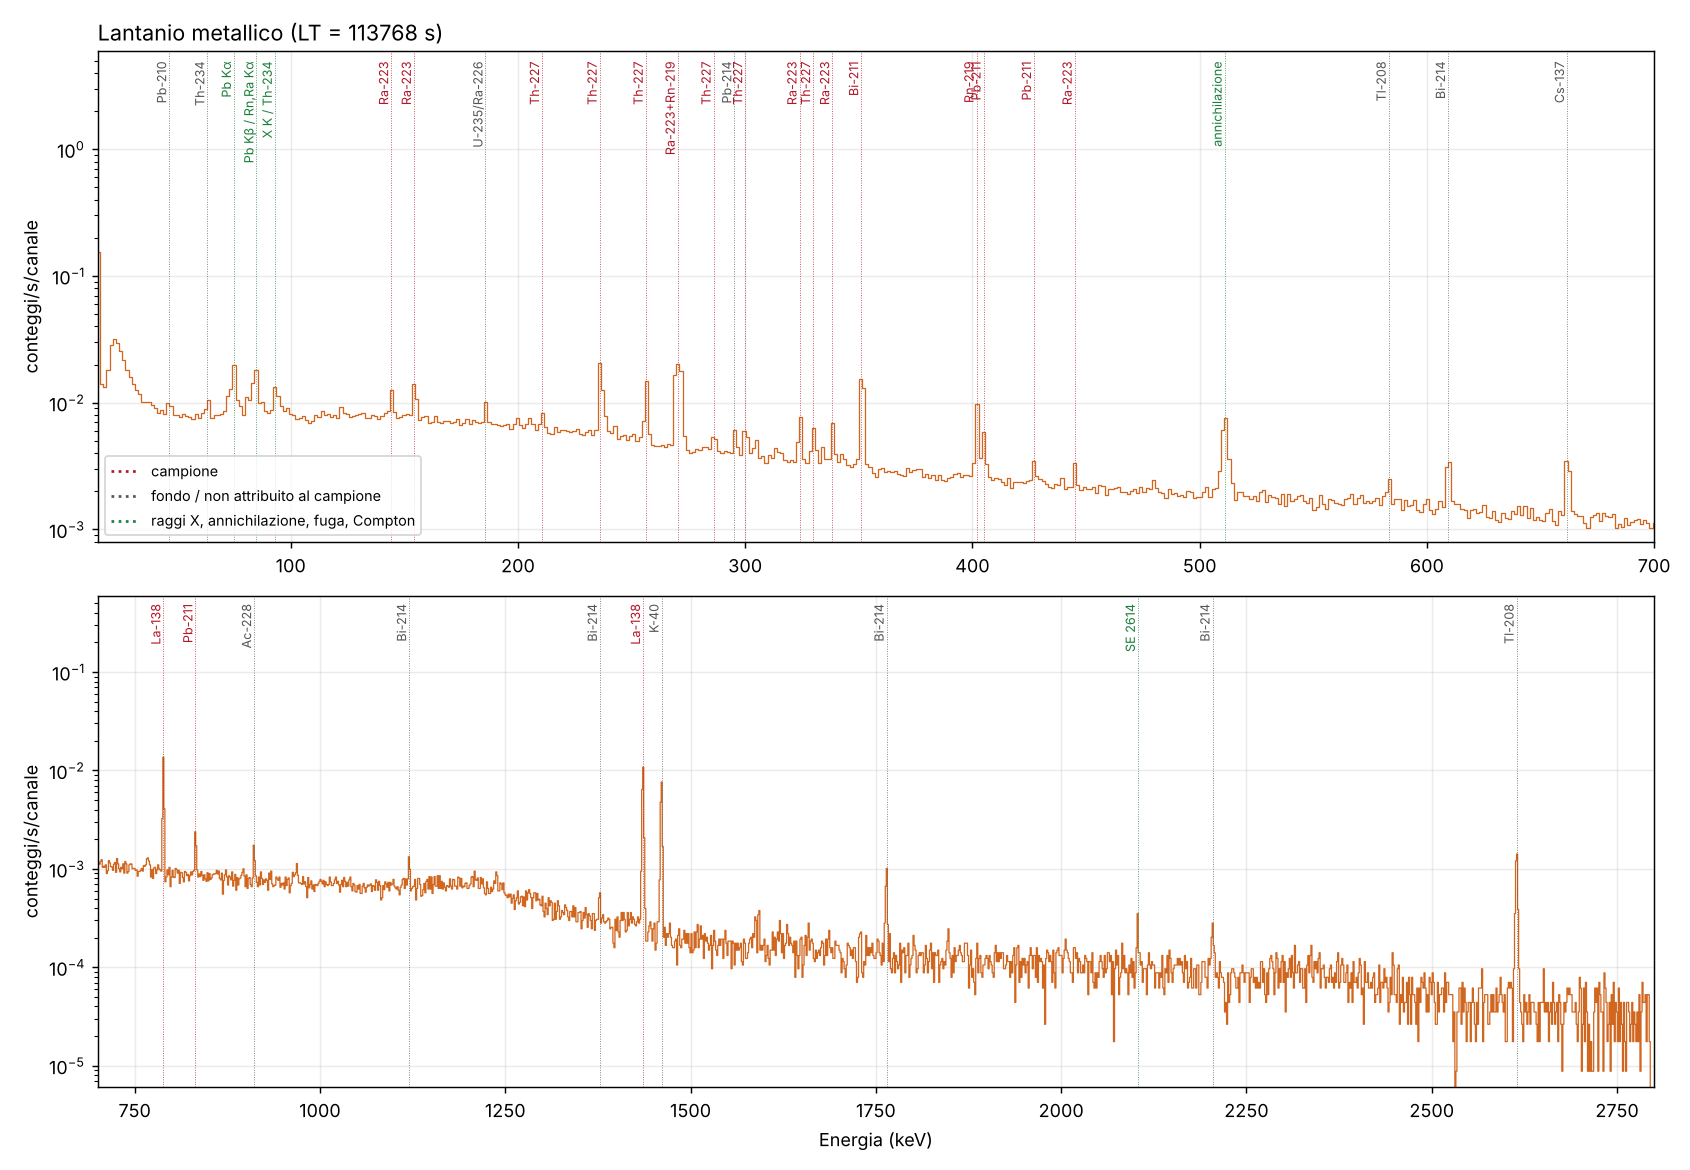
\includegraphics[width=\textwidth]{fig1_spettro_lantanio.png}
\caption{Spettro del lantanio metallico, normalizzato al live time.}
\end{figure}

\subsection{Contenuto: \nuc{138}{La} e catena dell'\nuc{227}{Ac}}

\begin{table}[H]
\centering\small
\begin{tabularx}{\textwidth}{llXX}
\toprule
Nuclide & $T_{1/2}$ & Linee osservate [keV] & Tassi netti [mcps]\\
\midrule
\nuc{138}{La} & $1{,}03\ee{11}$\,a & 788,74 ($\beta^-\to$\nuc{138}{Ce}); 1435,80 (CE $\to$\nuc{138}{Ba}) & $18{,}1\pm0{,}4$; $19{,}2\pm0{,}4$\\
\nuc{227}{Th} & 18,7\,d & 235,96; 256,23; 329,85; 210,6; 286,1; 304,5; 334,4 & 22,3; 12,8; 3,4; 2,9; 1,8; 1,6; 1,3\\
\nuc{223}{Ra} & 11,4\,d & 269,46; 154,21; 144,23; 323,87; 338,28; 445,03; 122,3 & 22,6; 9,6; 6,0; 5,4; 4,3; 1,4; 1,5\\
\nuc{219}{Rn} & 3,96\,s & 271,23; 401,81 & 20,0; 8,8\\
\nuc{211}{Pb} & 36,1\,min & 404,85; 427,09; 831,96 & 4,4; 1,6; $2{,}46\pm0{,}21$\\
\nuc{211}{Bi} & 2,14\,min & 351,06 & $\approx19^{*}$\\
raggi X K & --- & $\sim$81--94 (Rn/Ra); Pb K$\alpha$/K$\beta$ (schermo) & qualitativo\\
\bottomrule
\end{tabularx}
\caption{Nuclidi identificati nel lantanio metallico. Tutte le linee elencate hanno significatività $>5\sigma$. ${}^{*}$Il \nuc{211}{Bi} a 351,06\,keV non è risolto dal \nuc{214}{Pb} a 351,93\,keV. Il contributo del \nuc{214}{Pb} è stimato dalla sua linea a 295,2\,keV nello stesso spettro.}
\label{tab:catenaLa}
\end{table}

La presenza di \nuc{227}{Ac} nel lantanio è ben documentata. Ac e La sono chimicamente quasi indistinguibili, e l'\nuc{227}{Ac}, che appartiene alla serie del \nuc{235}{U}, segue il La nei minerali e nella purificazione. L'esempio classico è il fondo intrinseco degli scintillatori LaCl$_3$(Ce) e LaBr$_3$(Ce)~\cite{hartwell2005,milbrath2005,pnnl15453,labr2020}.

\begin{figure}[H]
\centering
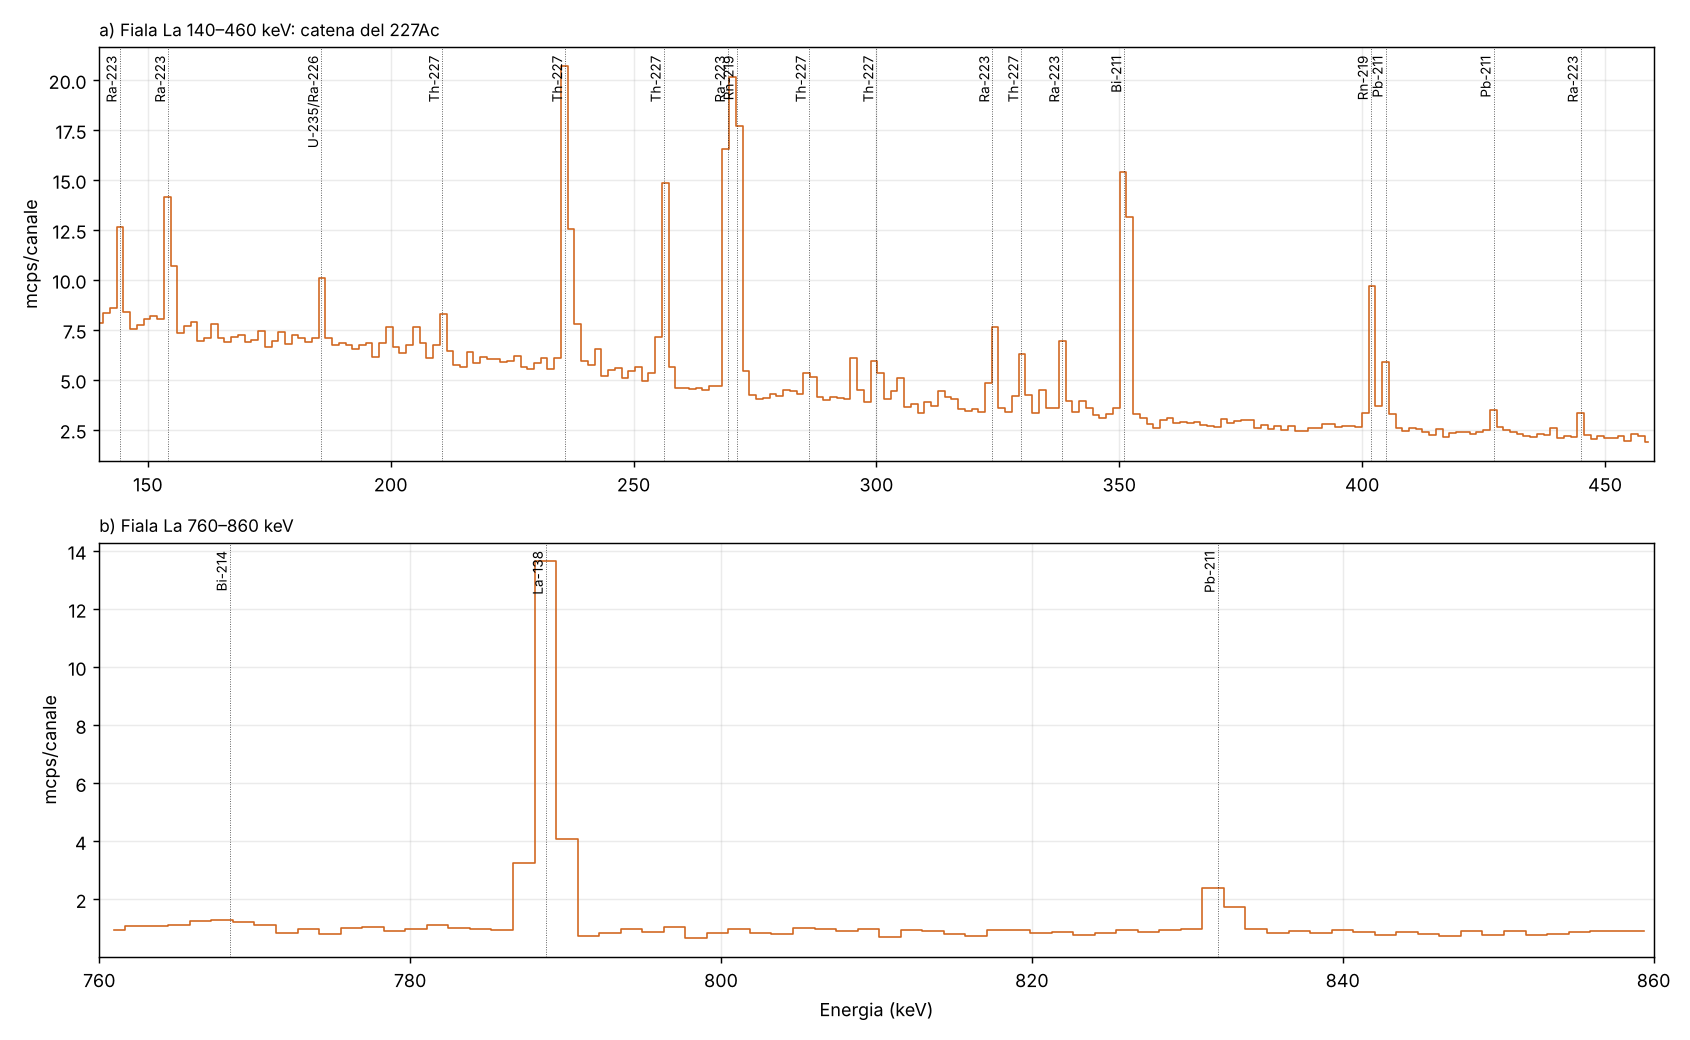
\includegraphics[width=\textwidth]{fig3_zoom_lantanio.png}
\caption{Lantanio metallico: (a)~regione 140--460\,keV con la catena dell'\nuc{227}{Ac}; (b)~\nuc{138}{La} a 788,7\,keV e \nuc{211}{Pb} a 832\,keV.}
\end{figure}

\subsection{Equilibrio della catena e autoassorbimento}

Con le linee della catena si costruisce una curva di efficienza relativa, con $\ln\varepsilon$ lineare in $\ln E$. Le linee del \nuc{227}{Th} e del \nuc{223}{Ra} cadono sulla stessa curva entro il 10--20\%, senza scarti sistematici fra le due famiglie.

Anche il \nuc{219}{Rn} a 401,8\,keV è in linea con la curva. In un metallo il \nuc{219}{Rn} ($T_{1/2}=3{,}96$\,s) non ha il tempo di diffondere fuori dal reticolo, quindi questo risultato è atteso.

Il quadro è compatibile con l'equilibrio secolare \nuc{227}{Ac}--\nuc{227}{Th}--\nuc{223}{Ra}--figli. Ne segue che il metallo è stato prodotto almeno alcuni mesi prima della misura, cioè circa 5--10 volte i 18,7\,d del \nuc{227}{Th}.

Il La metallico ha densità $6{,}15$\,g/cm$^3$ e $Z=57$, quindi attenua molto i fotoni di bassa energia. Questo contribuisce alla forte pendenza della curva di efficienza ($\varepsilon\propto E^{-0{,}54}$ tra 150 e 830\,keV). Poiché la curva è costruita con le linee dello stesso campione, l'autoassorbimento è già incluso nella calibrazione, purché \nuc{227}{Ac} e La siano distribuiti uniformemente nel metallo. Questo è ragionevole per un'impurezza chimicamente omologa.

\subsection{Livello di contaminazione da \nuc{227}{Ac}}

\paragraph{Riferimento interno.}
Con composizione isotopica naturale, il \nuc{138}{La} ha un'attività specifica nota:
\[
a(\nuc{138}{La}) = \frac{N_A}{M_\mathrm{La}}\,\theta_{138}\,\frac{\ln2}{T_{1/2}}
= \frac{6{,}022\ee{23}}{138{,}905}\cdot 8{,}881\ee{-4}\cdot\frac{\ln 2}{1{,}03\ee{11}\,\mathrm{a}}
\simeq 0{,}82\ \mathrm{Bq/g\ di\ La}.
\]

\paragraph{Rapporto di attività.}
Le efficienze a 789\,keV (\nuc{138}{La}) e a 832\,keV (\nuc{211}{Pb}) differiscono solo di circa il 5\%, per cui il confronto fra queste due linee dipende poco dalla curva di efficienza. Si ottiene:
\begin{itemize}
\item $A(\nuc{227}{Ac})/A(\nuc{138}{La})=\mathbf{1{,}38\pm0{,}12}$, confrontando direttamente le due linee;
\item $1{,}69\pm0{,}19$, usando l'intera catena con la curva di efficienza relativa.
\end{itemize}
La differenza fra i due valori fornisce una stima dell'incertezza sistematica.

\paragraph{Contenuto di \nuc{227}{Ac}.}
Ne seguono
\[
a(\nuc{227}{Ac})\approx1{,}1\text{--}1{,}4\ \mathrm{Bq\ per\ grammo\ di\ La\ (di\ metallo)},
\qquad
\frac{N_\mathrm{Ac}}{N_\mathrm{La}}\approx(2{,}6\text{--}3{,}2)\ee{-13}.
\]

Per confronto, la letteratura riporta $1{,}3\ee{-13}$ atomi della catena dell'\nuc{227}{Ac} per atomo di La in uno dei primi cristalli LaCl$_3$(Ce), e $5{,}8\ee{-15}$ in un LaBr$_3$(Ce) moderno~\cite{labr2020}. Il campione ha quindi un livello di \nuc{227}{Ac} tipico di un La commerciale non purificato specificamente dall'attinio.

\paragraph{Verifica di coerenza.}
Correggendo per le intensità, il rapporto fra le due linee del \nuc{138}{La} dà $\varepsilon(1436)/\varepsilon(789)=0{,}56$. L'estrapolazione della curva costruita sulla catena darebbe invece $0{,}73$. La differenza si spiega con due effetti:
\begin{itemize}
\item la curvatura della curva di efficienza sopra circa 850\,keV, non descritta dal modello lineare in $\ln E$;
\item la perdita per somma della linea a 1436\,keV con i raggi~X K del Ba emessi dopo la cattura elettronica.
\end{itemize}
Per questo il rapporto Ac/La è calcolato solo con la linea a 789\,keV.

\subsection{Altre linee}

Oltre alle linee del \nuc{138}{La} e della catena dell'\nuc{227}{Ac} (Tabella~\ref{tab:catenaLa}), nello spettro compaiono i picchi elencati nella Tabella~\ref{tab:altriLa}. Anche qui non restano picchi senza assegnazione.

{\small
\begin{longtable}{>{\raggedleft\arraybackslash}p{2.6cm}p{3.9cm}p{3.6cm}>{\raggedleft\arraybackslash}p{4.3cm}}
\caption{Lantanio metallico: picchi non appartenenti a \nuc{138}{La} o alla catena dell'\nuc{227}{Ac}.}\label{tab:altriLa}\\
\toprule
$E$ [keV] & Assegnazione & Note & Tasso [mcps]\\
\midrule\endfirsthead
\toprule
$E$ [keV] & Assegnazione & Note & Tasso [mcps]\\
\midrule\endhead
\bottomrule\endfoot
$<30$ & soglia del discriminatore & & ---\\
46,5 & \nuc{210}{Pb} & serie \nuc{238}{U} & $2{,}2\pm0{,}4$\\
63,3 & \nuc{234}{Th} & serie \nuc{238}{U} & $2{,}9\pm0{,}4$\\
72,8 / 75,0 & Pb K$\alpha_2$ / K$\alpha_1$ & fluorescenza dello schermo & $6{,}0\pm0{,}5$ / $13{,}9\pm0{,}5$\\
81--94 & raggi~X K di Rn e Ra + Pb K$\beta$ & conversione interna nella catena dell'\nuc{227}{Ac} & qualitativo\\
185,7 & \nuc{235}{U} + \nuc{226}{Ra} & & $3{,}6\pm0{,}3$\\
238,6 & \nuc{212}{Pb} & & $2{,}9\pm0{,}3$\\
242,0 / 295,2 / 351,9 & \nuc{214}{Pb} & & $1{,}4$ / $2{,}05\pm0{,}27$ / ---\\
511,0 & annichilazione + \nuc{208}{Tl} 510,8 & & $11{,}2\pm0{,}4$\\
583,2 / 2614,5 & \nuc{208}{Tl} & & $1{,}19\pm0{,}20$ / $3{,}27\pm0{,}18$\\
609,3 / 1120,3 / 1238,1 & \nuc{214}{Bi} & & $3{,}72\pm0{,}26$ / $1{,}03\pm0{,}16$ / $0{,}56\pm0{,}15$\\
1377,7 / 1764,5 / 2204,2 & \nuc{214}{Bi} & & $0{,}49\pm0{,}11$ / $1{,}69\pm0{,}14$ / $0{,}49\pm0{,}09$\\
661,7 & \nuc{137}{Cs} & origine non determinabile & $4{,}0\pm0{,}3$\\
911,2 / 969,0 / 1588,2 & \nuc{228}{Ac} & & $1{,}54\pm0{,}18$ / $0{,}79\pm0{,}18$ / $0{,}29\pm0{,}08$\\
$\sim$1219 & spalla Compton del 1435,8 (\nuc{138}{La}) & non è un picco & ---\\
1460,8 & \nuc{40}{K} & & $14{,}0\pm0{,}4$\\
1592,5 / 2103,5 & doppia / singola fuga del 2614,5 & & $0{,}40\pm0{,}09$ / $0{,}38\pm0{,}08$\\
\end{longtable}
}

\begin{itemize}
\item Il \nuc{137}{Cs} non appartiene né al \nuc{138}{La} né alla catena dell'\nuc{227}{Ac}. Senza uno spettro di fondo non si può stabilire se provenga dal campione o dall'ambiente di misura.
\item Le linee delle serie U e Th, il \nuc{40}{K} e i raggi~X del Pb sono quelle di un normale fondo di laboratorio e non sono quantificate.
\end{itemize}

%=====================================================================
\section{Conclusioni}

\paragraph{Trinitite.}
\begin{itemize}
\item Contiene \nuc{137}{Cs} (dominante), \nuc{241}{Am}, \nuc{152}{Eu}, \nuc{133}{Ba} e \nuc{239}{Pu}. Il \nuc{239}{Pu} è identificato dalle linee a 51,6 e 129,3\,keV.
\item \nuc{60}{Co}, \nuc{154}{Eu} e \nuc{155}{Eu} non sono rivelabili, come atteso dopo 81~anni di decadimento.
\item Rapporti di attività riportati alla data della detonazione:\\ $A(\nuc{137}{Cs})/A(\nuc{152}{Eu})=5{,}7\pm0{,}3$ (stat.);\quad $A(\nuc{133}{Ba})/A(\nuc{152}{Eu})=0{,}40\pm0{,}08$.
\item Lo spettro è compatibile con la trinitite del test Trinity descritta in letteratura.
\end{itemize}

\paragraph{Lantanio metallico.}
\begin{itemize}
\item È lantanio di composizione isotopica naturale, identificato dalle linee del \nuc{138}{La} a 788,7 e 1435,8\,keV.
\item È contaminato da \nuc{227}{Ac} in equilibrio secolare con i figli (\nuc{227}{Th}, \nuc{223}{Ra}, \nuc{219}{Rn}, \nuc{211}{Pb}, \nuc{211}{Bi}).
\item $A(\nuc{227}{Ac})/A(\nuc{138}{La})\approx1{,}4$--$1{,}7$,\\ cioè circa $1{,}1$--$1{,}4$\,Bq di \nuc{227}{Ac} per grammo di La, pari a $N_\mathrm{Ac}/N_\mathrm{La}\approx3\ee{-13}$.
\item Nello spettro è presente anche \nuc{137}{Cs}, di origine non determinabile.
\end{itemize}

\section{Limiti e misure consigliate}
\begin{itemize}
\item \textbf{Fondo:} per ciascuna configurazione di misura serve uno spettro a vuoto di almeno un giorno. Permetterebbe di sottrarre \nuc{40}{K}, U/Th ed eventuale \nuc{137}{Cs} ambientale, e di quantificare i radionuclidi naturali della trinitite.
\item \textbf{Efficienza assoluta, trinitite:} una sorgente multi-\gam{} certificata nella stessa geometria, oppure un calcolo Monte Carlo, insieme alla massa del frammento, permetterebbe di convertire i rapporti in Bq/g.
\item \textbf{Efficienza assoluta, La:} pesando il pezzo di La si ottiene direttamente l'attività del \nuc{138}{La}, $A=0{,}821\,\mathrm{Bq/g}\times m$. Da questa segue l'efficienza assoluta a 789\,keV e quindi l'attività dell'\nuc{227}{Ac} in Bq.
\item \textbf{Canali:} 2048 canali su 2,8\,MeV sotto-campionano i picchi. Conviene acquisire con 8192--16384 canali.
\item \textbf{Pu:} una quantificazione affidabile di \nuc{239+240}{Pu} richiede spettrometria $\alpha$ dopo separazione radiochimica~\cite{parekh2006,core}.
\end{itemize}

\begin{thebibliography}{99}\small
\bibitem{parekh2006} P.P.~Parekh, T.M.~Semkow, M.A.~Torres et al., \emph{Radioactivity in Trinitite six decades later}, J.~Environ.\ Radioact.\ \textbf{85} (2006) 103--120. \url{https://ui.adsabs.harvard.edu/abs/2006JEnvR..85..103P}
\bibitem{belloni2011} F.~Belloni, J.~Himbert, O.~Marzocchi, V.~Romanello, \emph{Investigating incorporation and distribution of radionuclides in trinitite}, J.~Environ.\ Radioact.\ \textbf{102} (2011) 852--862. \url{https://publications.jrc.ec.europa.eu/repository/handle/JRC67348}
\bibitem{nist2021} \emph{Gamma and Decay Energy Spectroscopy Measurements of Trinitite}, Nucl.\ Technol.\ (2021); arXiv:2103.06240. \url{https://arxiv.org/abs/2103.06240}
\bibitem{core} \emph{Measurements of radioactive gamma emitters in trinitites}. \url{https://core.ac.uk/works/146279469}
\bibitem{jrnc2013} Gamma spectrometry of 49 bulk trinitite samples, J.~Radioanal.\ Nucl.\ Chem.\ \textbf{295} (2013) 2049--2057, doi:10.1007/s10967-012-2201-4.
\bibitem{hartwell2005} J.K.~Hartwell, R.J.~Gehrke, \emph{Observations on the background spectra of four LaCl$_3$(Ce) scintillation detectors}, Appl.\ Radiat.\ Isot.\ \textbf{63} (2005) 223--228.
\bibitem{milbrath2005} B.D.~Milbrath et al., \emph{Characterization of alpha contamination in lanthanum trichloride scintillators using coincidence measurements}, PNNL (2005).
\bibitem{pnnl15453} PNNL-15453, \emph{Contamination in LaCl$_3$:Ce scintillators}. \url{https://www.pnnl.gov/main/publications/external/technical_reports/PNNL-15453.pdf}
\bibitem{labr2020} \emph{Intrinsic radiation background of LaBr$_3$(Ce) detector via coincidence measurements and simulations}, arXiv:2007.07552.
\bibitem{la138} \nuc{138}{La}: ENSDF/NNDC, \url{https://www.nndc.bnl.gov/ensnds/138/La/adopted.pdf}; DDEP (Bé et al.): CE 65,2(6)\,\%, $\beta^-$ 34,8(6)\,\%.
\bibitem{nucdata} Energie e intensità \gam: NNDC/ENSDF (NuDat) e DDEP/LNHB, \emph{Recommended Data}.
\end{thebibliography}

\noindent\footnotesize\textit{Nota sulle fonti:} i testi integrali di \cite{parekh2006,belloni2011,nist2021,core,jrnc2013} non erano scaricabili dall'ambiente di calcolo. Le affermazioni attribuite a questi lavori si basano su abstract e record indicizzati, e per questo non sono riportati confronti numerici con le loro tabelle di attività.

\end{document}
